\begin{figure}[!ht]
\centering
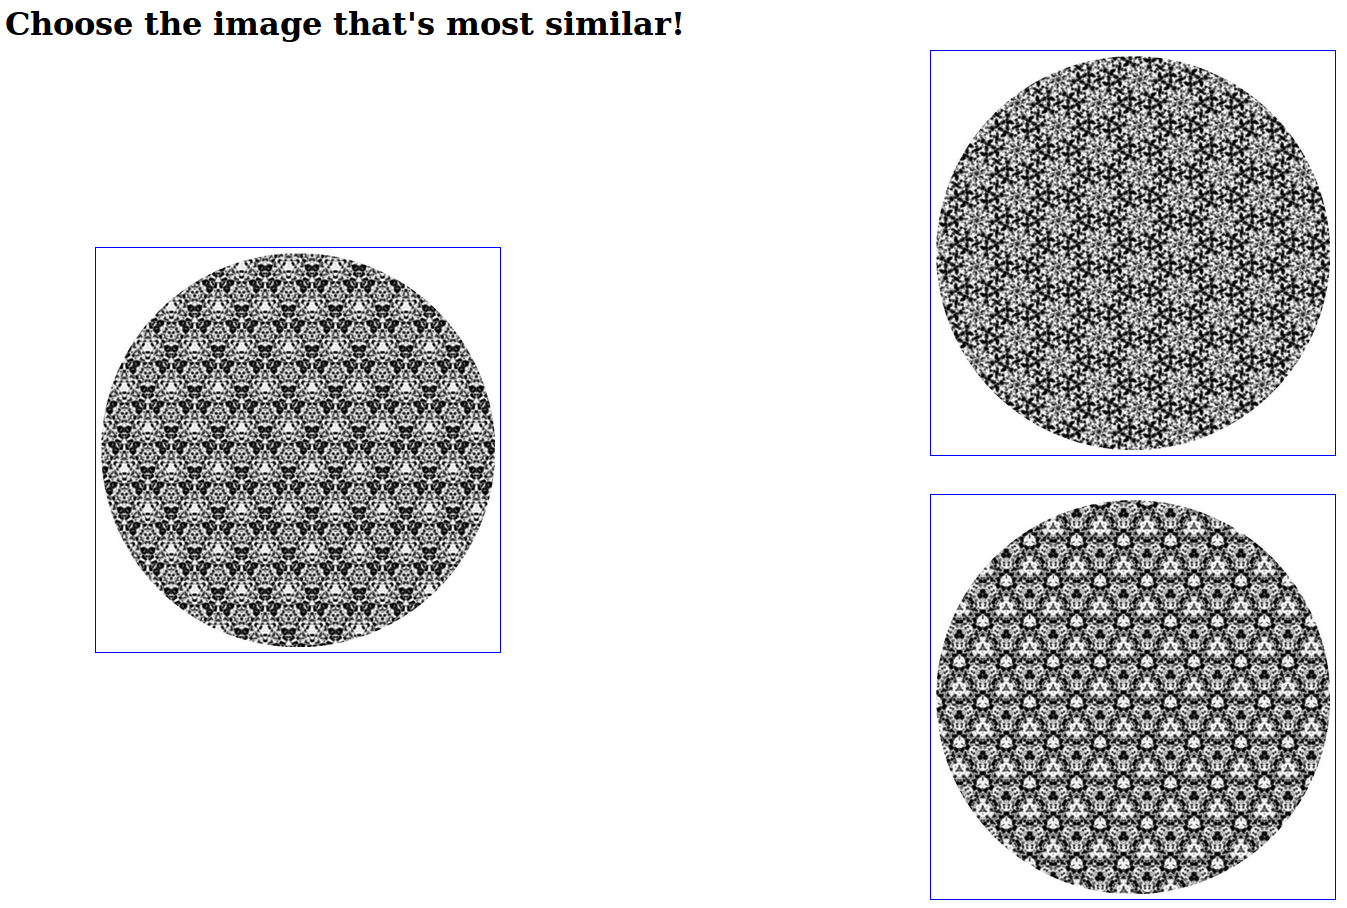
\includegraphics[width=0.9\columnwidth]{symper}
\caption{A screenshot of the experimental task}
\label{screenshot}
\end{figure}

\section{Experiments}
We designed an experiment where people had to distinguish between wallpaper groups. The goal of the task is to see which groups subjects can easily distinguish among and which groups are more challenging. In every trial, a subject was presented with two images from the same group and a third from one of the other sixteen groups. On the left, we have the \textit{target} image, which is the image with which they compare the other two images to. On the right, there is the \textit{goal} image, which always has the exact same group as the target image. Also, on the right is the \textit{distracter} image, which has any other wallpaper group. Figure~\ref{screenshot} shows what a single trial looks like. 

We recruited 106 participants on Mechanical Turk to participate in the experiment for compensation. Each subject performed 272 trials. This allowed each trial to have every group as the distracter image for every other group. This allows us to determine which features of the groups cause difficulty.

To generate these 272 tasks, we created every possible combination task from a small set of images from each wallpaper group. Then, each participant who accepted the HIT on Mechanical Turk was assigned a set of tasks randomly, though they received exactly one task that had any given group for the goal and the distracter.

We introduced a time limit of five seconds to ensure that the subjects were performing the task intuitively without relying on formal knowledge. This should give participants plenty of time to click the one they felt was more similar. However, when the task was given to people who have been trained in distinguishing wallpaper groups, they reported that the time limit felt too short to determine which group was which. Thus, it is likely that the results are a result of perception rather than education.

As the task can be tiring, subjects were allowed one break halfway through the experiment. Each subject was paid \$2 and a bonus for each task they successfully completed beyond chance, to encourage people to try as hard as they could on the task, instead of simply guessing. They could earn up to \$2 by answering 100\% correctly.  

Unfortunately, this incentive did not work on all participants. We excluded 10 participants from the analysis due to behavior that seemed consistent with either a lack of effort or following the directions poorly.  We used exclusion heuristics that identified participants that primarily clicked on either the top or bottom image, or if participants let a large portion of their tasks time out.


% We used three exclusion heuristics:

% \begin{enumerate}
% \item{A participant clicked the top or the bottom image more than 60\% of the time. If this was due to the system’s task generation, the probability of it occurring would be extremely low, about 0.001\%. However, 5/106 participants fell into this category, implying that their guessing strategy was slightly biased.}

% \item{A participant had more than 20\% of their tasks time out. Over-
% all, the rate of time out (exceeeding the five second time limit) was fairly low, around 4\%. Therefore, those participants with significantly higher rate of time outs either did not understand the task correctly or were not taking the task seriously. Only 4/106 participants fell into this category.}

% \item{If the system registered that a participant clicked more than 125\% of the number of tasks. Each task only required a single click to complete, so the assumption is that someone who is clicking that often is not actually looking at the images before clicking. Generally, this refers to clicks on the image. While some people have a more ``excitable'' clicking strategy, the average number of clicks was around 274, with the mode being 272. Those with significantly more were most likely clicking before the images loaded. Only 1/106 participants fell into this category.}
% \end{enumerate}

